
\documentclass[a4paper,11pt]{article}
\usepackage[T1]{fontenc}
\usepackage[utf8]{inputenc}
\usepackage[italian,english]{babel}
\usepackage[xindy]{imakeidx}
\usepackage{graphicx}
\usepackage[hidelinks]{hyperref}
\usepackage{caption}
\captionsetup{tableposition=top, figureposition=bottom, font=small}

\usepackage{epigraph}

\makeindex


\includeonly{sezioni/PrimiPassiNelWeb,%
			sezioni/IlSitoWeb,%
			sezioni/ProblemiDiUsabilita,%
			%sezioni/SitiEcommerce,%
			%sezioni/IlComportamentoDegliUtenti,%
			%sezioni/LaPubblicità,%
			%sezioni/LaRicerca,%
			%sezioni/IlNomeGiusto,%
			%sezioni/ProblematicheDellInformazione,%
			sezioni/MobileWeb,%
			%sezioni/SocialWeb,%
			%appendici/EyeTrackIII,%
			%appendici/WebSpamTaxonomy,%
			%appendici/LOD,%
			%appendici/ScrivereRelazioneUsabilita,%
			%appendici/AffrontareEsame%
			}
		
\begin{document}

\title{Appunti di Tecnologie Web 2}
\author{Eduard Bicego}
\date{2016}

\maketitle

\begin{abstract}
	`` .''
\end{abstract}

\tableofcontents
	\newpage
\listoffigures




\section{Primi passi nel Web}
	
	\subsection{1945 Memex}
		
	\subsection{1960-68 NLS: onLine System}
		
	\subsection{1960 Xanadus}
		
	\subparagraph*{Morale}
			\begin{quote}
				``I sistemi sociali "Open World" devono essere gratis.''
			\end{quote}
		
	\subsection{1980 Enquire}
		
	\subsection{1990 World Wide Web}
		
	\subsection{Le alternative al WWW}



\chapter{Il sito Web}

	\section{La metafora del negozio}
		Possiamo considerare qualsiasi sito web come una casa o meglio un negozio: la gente guarda e poi decide se comprare o andarsene.
		L'\textbf{homepage} è la vetrina del negozio in cui le persone cercano informazione e questa informazione deve essere usufruibile nel modo più efficace possibile. A tal proposito sorge il problema di comunicare nei migliori dei modi l'informazione, un problema fortunatamente già affrontato dal giornalismo. Il pezzo informativo perfetto è il risultato dei 5 assi informativi principali, le così dette \emph{5 W} (\emph{6 W}): Where - Who - Why - What - When (- How).
		Che nel web si traducono rispettivamente in:
		\begin{description}
			\item[Where] A quale sito sono arrivato?
			\item[Who] Chi c'è dietro questo sito?
			\item[Why] Perché sono qui? Quale benefici mi dai?
			\item[What] Che cosa mi offri? Mostramelo.
			\item[When] Ultime novità del sito.
			\item[How] Capito questo, come arrivo a quello di mio interesse?
		\end{description}
	
	\section{Problemi e implicazioni}
		Il principale problema di un utente che visita il sito è il \textbf{TEMPO}. Bisogna sempre considerare che gli utenti hanno:
			\begin{itemize}
				\item aspettative.
				\item poco tempo, secondi contati!
			\end{itemize}
		Il sito quindi deve sapere offrire le \emph{6 W} nel pochissimo tempo che l'utente gli dedica.	L'utente medio all'arrivo sulla homepage ha circa \textbf{31 secondi} prima di cominciare ad avere sensazioni negative. 31 secondi. Solo 31 secondi per convincere l'utente. Questo porta ad una serie di implicazioni:
		
			\subsection{Quanto testo nella homepage?} Un uomo adulto di buona cultura legge dalle 200 alle 300 parole al minuto, su monitor però la velocità di lettura è più bassa: circa 180 parole al minuto. Facendo un po' di conti con più di 93 parole abbiamo già superato il limite di 31 secondi, se teniamo poi conto dei secondi investiti sul layout allora 93 parole sono decisamente troppe.
			\subsection{Il comportamento dell'utente è dinamico} Bisogna far sì che l'utente al nostro sito ci ritorni ma ora le W di Who, Where e Why non sono più richieste. Fortunatamente l'utente salta alcuni pezzi ma ora ha ancora meno tempo da dedicare.
			
		\subsection{Questione di tempo}	
			Di seguito i tempi medi di permanenza:
			\begin{itemize}
				\item 1ª volta: 31 secondi.
				\item 2ª volta: 25 secondi.
				\item 3ª volta: 22 secondi.
				\item 4ª volta: 19 secondi.
				\item dalla 5ª volta in poi i tempi sono stabili.
			\end{itemize}
			Dalla seconda volta in poi quello è il patrimonio dei secondi da dedicare agli assi What, When e How, corrispondono a 57 parole al massimo!
			Una home prolissa non darà mai tutti gli assi informativi nei pochi secondi a disposizione e una home poco chiara (assi informativi mancanti) darà un motivo in più per scappare all'utente.
			
		\subsection{E il resto del sito?}
			Per tutte le altre pagine non abbiamo bisogno che gli assi siano il principale obiettivo informativo. Inoltre l'utente una volta superata la homepage (vetrina) dedica più tempo. Dai 31 secondi passa a \textbf{53 secondi} che corrispondono a circa 160 parole in cui includere info più specifiche.
			Un ottimo modo per gestire il poco numero di parole è quello di attirare l'attenzione dell'utente con descrizioni corte che conducano ad altre pagine per ulteriori informazioni, ciò fa sì che solo l'utente effettivamente interessato leggerà il testo più lungo mentre agli altri verrà fatto perdere meno tempo.
			Sembrerebbe un'ottima soluzione quella di spezzare la pagina e resettare i timer guadagnando tempo ma attenzione perché oltre al tempo singolo di ogni pagina bisogna considerare anche il \textbf{tempo globale}.
			
		\subsection{Questione di tempo - Parte II}
			Il \textbf{tempo globale} rappresenta il tempo massimo dell'utente per raggiungere lo scopo. Si suddivide in due:
			\begin{description}
				\item[Tempo preliminare:] è il tempo che un utente dedica per convincersi a restare nel sito, per questo chiamato anche \textbf{tempo di scelta}. Il tempo di scelta medio è di 1 minuto e 50 secondi, allo scadere di questo timer l'utente abbandona il sito indipendentemente se esso conteneva l'informazione ricercata o no. Nell'88\% dei casi quell'utente non ritornerà più.
				\item[tempo complessivo:] l'utente è convinto a restare per cui dedica fino a 3 minuti e 49 secondi per avere successo altrimenti abbandona.
			\end{description}
			
			\subparagraph*{Morale:}
			\begin{quote}
				``È molto importante il bilanciamento tra homepage e pagine interne.''
			\end{quote}
			Al primo accesso infatti l'utente dopo aver navigato homepage e una pagina interna decide se restare o andarsene (1:50 - tempo di scelta). Dopo tre pagine e mezzo l'utente deve aver successo in quello che doveva fare.
	
	\section{L'importanza della struttura}
		Riassumiamo quanto detto.
		\begin{itemize}
			\item Dopo un click l'utente deve essere convinto a restare.
			\item Dopo tre link l'utente deve avere quello che cercava.
		\end{itemize}
		
		Ora nelle pagine interne che assi informativi servono? Sembrerebbe che non serva replicare le info della home page nelle pagine interne ma la navigazione al giorno d'oggi non attraversa quasi mai la home page!
		Grazie ai motori di ricerca infatti la navigazione può cominciare da qualunque punto di qualsiasi sito.
	
		\subsection{Deep linking}
			Questo fenomeno viene chiamato \textbf{deep linking} ovvero avere il link interno di un sito. Accade questo perché anche i motori di ricerca hanno i loro timer e devono dare nel modo più diretto l'informazione giusta che l'utente cerca.
		Ogni pagina quindi può essere una pagina iniziale per un utente. La metafora del negozio si fa critica perché ciò significherebbe avere clienti teletrasportati all'interno, già tra gli scaffali.
		
		\subsection{Gli assi in dettaglio}
			Andiamo quindi a vedere gli assi in dettaglio e come bisogna gestirli in seguito al \emph{deep linking}.
			Alcuni assi risultano essere \textbf{obbligatori} per tutte le pagine:
			\begin{itemize}
				\item Who: il logo (solitamente da preferire in alto a sinistra).
				\item What: tipicamente un link alla home page.
			\end{itemize}
			Altri risultano essere \textbf{opzionali}:
			\begin{itemize}
				\item When: le novità del sito.
			\end{itemize}
			Altri ancora entrano nella categoria \textbf{opzionali consigliati}:
			\begin{itemize}
				\item Why: basta una breve descrizione, uno slogan.
				\item How: funzionalità di search (da preferire in alto a destra).
			\end{itemize}
		
		\subsection{L'importanza del Where}
			Un paragrafo a parte invece è doveroso dedicarlo all'asse Where. Infatti in ogni pagina si dovrebbe rendere chiaro il contesto in cui l'utente si trova. Si potrebbe obiettare con "perché non mandarlo alla home page?" come per l'asse What ma ciò costituirebbe un link in più all'utente e, peggio, spostare l'utente dal luogo in cui c'è l'informazione di suo interesse. Conviene dargli informazioni del Where nella pagina interna.
				Per fare questo si utilizza il \emph{breadcrumb}, ne esistono di tre tipi:
				\begin{description}
					\item[Location:] dà il posto della pagina nella gerarchia del sito. Ad esempio: "Home >> Categoria >> Pubblicità >> Pagina".
					\item[Attribute:] mostra la categoria e gli attributi della pagina. Un po' come gli hashtag odierni. Una pagina può trovarsi sotto più categorie.
					\item[Path:] mostrano il cammino dell'utente per giunger alla pagina. È dinamico infatti dipende dal cammino dell'utente e usa dei \emph{cookie} per tenere traccia di tali informazioni.
				\end{description}
				
				\paragraph{Pro e contro}
					\begin{itemize}
						\item \textbf{Location} non risolve il problema del Where dopo che l'utente è catapultato nella pagina.
						\item \textbf{Attribute} sembra la scelta migliore ma implica un sistema più complesso per gestire il sito e raggiunge taglie troppo grandi in certi casi.
						\item \textbf{Path} resta una soluzione semplice e lineare.
					\end{itemize}
				
				\paragraph{Separatori}
					Per completezza si riportano i separatori per \emph{breadcrumb} più comuni:
					\begin{itemize}
						\item segno di maggiore \verb|>|;
						\item segno di doppio maggiore \verb|>>|;
						\item backslash \verb|\|;
					\end{itemize}
				


\section{Problemi di usabilità}

	\subsection{Problemi persistenti}
		Sono i problemi gravi fortemente connessi alla tecnologia e che nel tempo non cambieranno.
	
		\subsubsection{Navigazione}
			Il problema del navigare nel web odierno è la possibilità di perdersi: \emph{lost in navigation}, ossia la prese di coscienza dell'utente che capisce di essersi perso. Fortunatamente, se opportunamente inserito, l'asse informativo Where risolve questo tipo di problema.
			\paragraph*{Morale:}
			\begin{quote}
				``Gli utenti devono essere coscienti di dove sono e dove devono andare.''
			\end{quote}
			
			\paragraph{Dove sono, dove ero e dove sarò}
				Nonostante l'uso di \emph{breadcrump} e asse Where opportunamente comunicato all'utente ciò non basta. Può infatti capitare che l'utente si ritrovi in pagine già visitate e deva ricordarsi i percorsi già fatti. Lo sforzo diventa pesante e crea malumore. Per non far affaticare l'utente esiste al giorno d'oggi una consuetudine non standard riconosciuta in tutto il web che è quella di colorare diversamente i colori dei link già visitati. Ciò fu implementato da Netscape Navigator e da allora è diventata una buona norma per garantire maggior usabilità.
				Il 75\% dei siti web usa il cambio colore dei link già visitati.
			\subparagraph*{Morale:}
			\begin{quote}
				``All'utente pesa meno la grafica rispetto alla funzionalità e allo sforzo.''
			\end{quote}	
			
		\subsubsection{I movimenti dell'utente}
			Le azioni generali per interagire che può utilizzare l'utente sono:
			\begin{itemize}
				\item il \emph{click}.
				\item il \emph{back} (pulsante prezioso, presto vedremo il perché).
			\end{itemize}
			Secondo gli studi sul comportamento degli utenti sul web si è scoperto che ad essi piace navigare all'indietro, anzi lo adorano. Prendiamo ad esempio la visita di un sito in cui si sia andati in profondità di 4 livelli e si deva tornare alla homepage. Gli utenti a questo punto spesso invece di cliccare una volta  il link diretto (magari sul logo del sito) preferiscono di gran lunga utilizzare il pulsante \emph{back} ripetutamente.
			Si arriva fino a 7 click del pulsante \emph{back} anche in presenza di un link diretto. È lo stesso comportamento che si tiene con il telecomando della propria TV. A volte basterebbe premere i pulsanti numerici per passare ad un diverso canale ma si preferisce spostarsi di un canale alla volta usando un unico bottone invece di due o più bottoni numerici. Questo uso comune è noto come \emph{backtracking}.
			\subparagraph*{Morale:}
			\begin{quote}
				``La pulsione primaria dell'utente non è quella di minimizzare il tempo ma quella di minimizzare lo sforzo.''
			\end{quote}
			L'uomo ha orrore nello sforzo previsto nel futuro e tende a fare cose folli e illogiche per allontanare tale sforzo (si veda \emph{l'algoritmo della carta igienica}). Quindi, gli utenti minimizzano lo sforzo computazionale e per fare ciò ricorrono all'uso del pulsante \emph{back} perché:
			\begin{itemize}
				\item non serve ricordarsi il percorso;
				\item non bisogna trovare il tasto \emph{back}, (è sempre lì garantito).
			\end{itemize}
			Da ciò ovviamente ne consegue che non bisogna \textbf{mai togliere l'uso del \emph{back button}}
			
		\subsubsection{Nuova finestra? No, grazie}
			Un altro problema persistente è quello di aprire una nuova finestra di navigazione anziché usare sempre la stessa.  Esistono due tipi di finestre, il tab e la nuova finestra vera e propria. L'aprire una nuova finestra ha gravi conseguenze per l'utente medio:
			\begin{itemize}
				\item Non c'è più la cronologia di navigazione (addio \emph{back button}!
				\item Avere finestre diverse aperte confonde l'utente medio.
			\end{itemize}
			Analiziamo nel dettaglio che cosa susccede all'apertura di una nuova finestre. Prima di tutto questa si sovrappone alla navigazione esistente provocando panico per l'utente medio. Se dovesse non sovrapporsi l'utente medio seleziona quella bassa lasciando l'altra finestra aperta. Di conseguenza il link della pagina già aperta non funziona più perché la pagina risulta aperta ma di ciò l'utente medio non ne è a conoscenza.
			
			\paragraph{Un problema correlato: i pop-up}
				Un problema che si collega molto con l'apertura di una nuova finestra è quello dei pop-up. Piccole finestre che si aprono senza il permesso dell'utente (si veda in seguito per maggiori dettagli).
		
		\subsubsection{Convenzioni violate}
			Le convenzioni non sono standard ma semplicemente la prassi, ciò che fanno tutti e per questo più familiari all'utente. 
			
			\paragraph{Legge di Jacob}
			\begin{quote}
				``Gli utenti spedono la maggior parte del tempo su altri siti web."
			\end{quote}
			Gli utenti sono abituati a navigare in altri siti quindi non abbiamo il potere di fare tutto di testa nostra solo perché è il "nostro" sito.
			
		\subsubsection{Altri problemi: What non rispettato}
			Mai usare linguaggio vuoto o con poco contenuto/slogan. L'uente che visita una pagina si aspetta contenuto non ``politichese'' cit.
			
			\paragraph{Problema correlato: la forma del testo}
				Il contenuto di una pagina web conta ma il testo deve sempre avere una forma semplice, chiara e sintetica; la lettura su schermo è diversa dalla normale lettura su carta. Mai usare testo difficile e monolitico che spesso, purtroppo, è usato nei siti delle pubblica amministrazione. Il testo usato su altri media non è adatto al web. Alcuni accorgimenti per evitare ciò è quello di tagliare testo.
				\begin{itemize}
					\item Se abbiamo del normale testo da inserire in una pagina bisogna \textbf{dimezzare} per far sì che diventi testo web.
					\item Se abbiamo testo generico, il testo web è circa \textbf{un quarto}.
				\end{itemize}
				Un altro suggerimento per scrivere testo adatto al web è quello di cominciare con la conclusione e successivamente espandere.
	
	\subsection{Problemi non-persistenti / Il contenuto}
	
		\subsubsection{Splash page}
			Le \emph{splash page} Sono le pagine di presentazione che sostituiscono la homepage. Evitarle a tutti i costi, fanno perdere tempo all'utente soprattutto se sono anche animate. Molto meglio una homepage semplice che comunica in modo adeguato i 6 assi principali.
		\subsubsection{Richieste di registrazione}
			Altra cosa da evitare: mai richiedere informazioni personali all'utente, soprattutto mai richiedere una registrazione prematura. Su 10 utenti appena l'1,1 è disposto a dare la propria mail.	Bisogna infatti tenere conto di:
			\begin{itemize}
				\item l'utente deve sapere se vale la pena o no (problema di \emph{trust}).
				\item La registrazione richiede sforzo computazionale (nuova login e password!).
			\end{itemize}
			Alcuni siti arrivano pure a bloccare la prima visita con un pop-up richiedendo l'iscrizione. Come può un utente in questo modo capire se fidarsi on se non li è lasciata opportunità di visitare prima il sito? Ogni richiesta di registrazione deve avvenire dopo aver convinto l'utente.
			
		
		\subsubsection{Lo scrolling maledetto}
			Parliamo di \emph{scroll} verticale. I dati mostrano che in media gli utenti "\emph{scrollano}" 1.3 schermi. Questo significa che in totale la parte visualizzata di una pagina corrisponde a 2.3 schermi. Tutto quello che viene dopo (in media) non viene visto. Per cui, attenzione alla struttura del layout della pagina e alla posizione dei contenuti.
			\begin{itemize}
				\item Nella homepage solo il 23\% effettua lo \emph{scroll}.
				\item Nelle pagine interne il 42\%.
				\item Visite ripetute alla homepage riducono l'uso dello \emph{scroll} al 14\%.
			\end{itemize}
			Riportiamo l'esempio da non imitare dell'attuale (07/02/2016) pagina di presentazione dell'iPod nano: \url{http://www.apple.com/it/ipod-nano/}. Alcune osservazioni:
			\begin{itemize}
				\item All'apertura la figura in primo piano è tagliata (potrebbe essere un modo per incoraggiare lo scroll).
				\item Il testo anche se conciso non dice nulla di utile all'utente.
				\item La pagina è composta da 14 (!!!) \emph{scroll}.
			\end{itemize}
			
			\paragraph{Taglia dello schermo}
				Un gran gratta capo di oggi per i siti web è la taglia dello schermo (risoluzione). Ad oggi sono numerosissime. Negli anni passati 1024x768 era una taglia di riferimento ma con l'avvenuta dei netbook (1014x600 massima) il trend è cambiato. Inoltre non è detto che tutti massimizzino la finestra per cui statisticamente la taglia più sicura su cui affidarsi è la 800x600. Con il mobile le cose peggiorano. Non conta più la taglia dei pixel (risoluzione) ma dello schermo vero e proprio. Esistono infatti piccoli schermi con risoluzioni alte.
				Per risolvere questo problema troppo spesso si è ricorso al \emph{frozen layout} ossia fissare il design per una taglia con il risultato di avere effetti disastrosi con le taglie più grandi. Se si fissa l'asse orizzontale otterremo infatti con uno schermo grande una pagina piccola e contenuta con ovvio spreco di spazio con un schermo piccolo invece l'odiato \emph{scroll} orizzontale.
				
			\paragraph{Scrolling orizzontale}
				Lo \emph{scroll} orizzontale è odiato dagli utenti ed è molto peggio del verticale perché:
				\begin{itemize}
					\item non è comune
					\item e non rispetta la normativa classica del testo.	
				\end{itemize}
				Nella lettura l'asse delle ascisse è fissato mentre viene effettuato lo \emph{scroll} sull'asse delle ordinate con gli occhi. Inoltre avere entrambi gli \emph{scroll} porta a dover gestire uno spazio di 2 dimensioni con logica conseguenza di attivare più sforzo computazionale.
			
			\paragraph{People do scroll}
				Potrebbe essere interessante approfondire la questione dello \emph{scroll}. Da un lato abbiamo visto che lo \emph{scroll} è uno sforzo in più richiesto all'utente ma il tempo passa e il comportamento e le abitudini degli utenti possono cambiare (soprattutto il boom mobile). Ci sono molti studi che indicano che gli utenti sono pronti a fare lo sforzo di \emph{scroll} se il layout lo incoraggia. Ulteriori approfondimenti \url{http://it.uxmyths.com/post/28647124262/mito-3-le-persone-non-scrollano}.
				
		\subsubsection{Lo sforzo computazionale spiegato da Engelbart}
			Abbiamo parlato nella sezione La storia del Web (\url(https://www.youtube.com/watch?v=1MPJZ6M52dI) della straordinaria invenzione di Douglas Engelbart dove oltre ad il primo mouse della storia si vedeva una tastiera da 5 tasti. Essa permetteva di memorizzare fino a 31 combinazioni di tasti associate ad un evento sulla macchina. Questa tecnologia non è sopravvissuta proprio per il troppo sforzo computazionale richiesto. Per questo motivo per ogni cosa chiedetevi sempre qual è lo sforzo che un utente deve compiere e cercate di minimizzarlo, l'uomo si muove sempre verso quella direzione.
		
		\subsubsection{Bloated design}
			Il \emph{bloated design}, letteralmente design gonfiato, è un altro tipico errore che abita il web odierno. Il \emph{bloated design} si ha quando il sito presenta troppi effetti, questo risulta essere \textbf{statisticamente fastidioso} poiché aumenta lo sforzo computazionale.
			Nella storia del web questo si è presentato con la lotta tra i \emph{browser} dove si creavano comandi con effetti bizzarri e inutili per l'utenza. Alcune anni dopo un comando di questi, il \emph{blink tag} fu definito dallo stesso autore come ``la cosa peggiore per internet".
			Di esempi di \emph{bloated design} ce ne sono centinaia:
			\begin{itemize}
				\item uso di musica con avvio automatico al caricamento.
				\item effetti sconvolgenti che confondono l'utente.
				\item siti di design in cui risulta complicata la navigazione.
				\item e altro ancora...
			\end{itemize}
		
		\subsubsection{Abusi multimediali}
			
			\paragraph{Il 3D - Prima, dopo, ora}
				Perché l'interfaccia 3D non è entrata nel mondo del web? Già nel 1922 fu proposto nella televisione ma non ebbe successo. Ancora una volta il limite dell'umano, la necessità di minimizzare lo sforzo computazionale determina il fallimento di una tecnologia proprio come la tastiera di Douglas Engelbart. 
				Non limitiamoci solo al web, perché non rendere l'interfaccia dei sistemi operativi in 3 dimensioni? Ci ha provato Anand Agarawala nel 2007, designer, (\url{https://www.ted.com/talks/anand_agarawala_demos_his_bumptop_desktop}) proponendo una interfaccia virtuale che simula la fisica in 3 dimensioni. Perché questa interfaccia non è ancora ne nostri dispositivi? La difficile interazione con esso si è rilevata più importante che ne la bellezza visiva.
				Se possiamo evitiamo l'uso smoderato della multimedialità, il sito commerciale J. Crew lo sapeva bene quando per mostrare i propri vestiti non ha usato nessuno effetto. Una scelta banale ma è quello che l'utente vuole.
				
				\subparagraph*{Morale:}
				\begin{quote}
					``Conviene offrire \emph{snapshot} 2D di oggetti 3D con complessità bassa"
				\end{quote}
				
			\paragraph{I plugin}
				Una nota per i \emph{plugin}: soffrono di un problema fondamentale, non sono standard e richiedono un'installazione quindi sforzo aggiuntivo. Il comportamento dell'utente di fronte alla richiesta dell'installazione di un \emph{plugin}:
				\begin{itemize}
					\item ``non so cosa può succedere quindi non lo faccio" (vedi gli aggiornamenti di Windows 10 ora nascosti all'utente).
					\item Installare un \emph{plugin} fa perdere tempo (una richiesta di installazione di plugin fa perdere il 90\% degli utenti non fidelizzati).
				\end{itemize}
			
			\paragraph{Dai plugin a Flash!}
				Si potrebbe pensare che con \emph{Flash} i problemi dei \emph{plugin} non si hanno più. Sbagliato!
				\begin{itemize}
					\item \emph{Flash} è sempre un \emph{plugin} con necessità costante di agigornamenti.
					\item Tempo di caricamento aumentato.
					\item Dà molti mezzi e più libertà espressiva, un vantaggio che diventa problema se si cade nel già visto \emph{bloated design}.
				\end{itemize}
				Evitare \emph{Flash} non significa evitare questi problemi. Anche con il recente HTML5 si può cadere in trappole come il \emph{bloated design}. Tutto dipende dall'uso.
			
			\paragraph{I video}
				Un altro strumento multimediale è l'uso dei video, oggi sempre più in espansione (si pensi a Facebook e al recentissimo Snapchat). Il principale vantaggio è lo stesso della televisione: basso costo computazionale. Di contro abbiamo la richiesta di più risorse (banda) e il timer collegato alla durata del video. 
				\begin{itemize}
					\item Tempo medio consigliato: 1 minuto.
					\item Tempo massimo consigliato: 2 minuti.
				\end{itemize}
				Questi sono consigli generali ma molto dipende dal \textbf{target} che si ha, ad esempio youtube non ha questi limiti.
		
		\subsubsection{La Metafora visiva}
			Altro problema che nel web produce disastri sull'usabilità dei siti web. La metafora visiva si ha quando l'utente è ingannato dall'aspetto grafico che dà aspettative illusorie e le tradisce. Per esempio:
			\begin{itemize}
				\item Il pulsante dello \emph{scroll} sostituito da un immagine.
				\item L'immagine con scritto "clicca" non cliccabile.
				\item Un testo in grassetto colorato che ricorda un link ma non lo è.
				\item Pulsanti non cliccabili.
				\item Immagini non riconosibili come immagini.
				\item Pulsanti che sono parzialmente cliccabili.
				\item ...
			\end{itemize}
			Le metafore visive tradite non hanno soltanto a che fare con link, pulsanti e immagini ma anche con \textbf{concetti}. Ad esempio dei concetti che significano qualcosa ma non sono intuibili subito.
		
		\subsubsection{I menu di navigazione}
			\paragraph{Pathfinding}
			\paragraph{Fault-tollerant}
			
		\subsubsection{Il testo}
			
			\paragraph{Caps lock}
			\paragraph{Immagini sostitutive}
			\paragraph{La maledizione Lorem Ipsum}
				\subparagraph{L'effetto ghigliottina}
				
		\subsubsection{Scanning}
			\paragraph{Strutturazione}
			\paragraph{Problemi}
			\paragraph{Blonde effect}		

%\include{sezioni/}

%\include{sezioni/}

%\include{sezioni/}

%\include{sezioni/}

%\include{sezioni/}

%\include{sezioni/}

%\include{sezioni/}

%\include{sezioni/}

%\include{sezioni/}


\section{Mobile Web (e App)}
	Solo recentemente i dispositivi mobile hanno spopolato è la tecnologia ha superato di gran lunga i web designer che sono impreparati nell'ambito mobile emergente. Nel 2013 l'accesso a internet da dispositivi mobile ha superato quello di desktop e laptop ed è in costante crescita. Nonostante questo trend, 530 siti nella top 1000 del mondo non dispongono di una versione mobile e il 25\% di questi sfora lo schermo.

	\subsection{Un po' di storia}
		Nel marzo 2013 avviene un importate scelta aziendale in Google. Il team di sviluppo di Android che non portava risultati soddisfacenti è inglobato dal team di Chrome che invece aveva successo. L'idea era ed è quella di avere convergenza tra mondo mobile e web. 
		
		Già prima si era cercato di percorrere questa rotta da Google ma le cose non andarono bene visti i contrasti con Apple che non voleva collaborare. Si pensi che lo stesso Steve Jobs era contrario alle app. Da qui il motivo dell'acquisto del sistema Android da parte di Google.
		
		Ora il percorso è ben delineato: la nascita delle hybrid apps scritte usando HTML5 e multipiattaforma segnano ancora più visivamente la convergenza tra mobile e web.
	
	\subsection{Le App}
		Nascono dalla necessità di minimizzare ancora una volta lo sforzo computazionale delle persone. L'app minimizza enormemente il tempo di accesso al servizio richiesto dagli utenti. Di conseguenza questo porta a maggiori esigenze da parte degli utenti e riduce i timer di soddisfazioni.
		
		\subsubsection{Parlano le statistiche}
			Dalle statistiche emerge:
			\begin{itemize}
				\item quasi un quarto degli utenti usano app più di 60 volte al giorno 
				\item e questo cresce ogni anno del 123\%!
				\item La fascia d'età che meno 'drogata' di app si trova tra i 25 e 35 anni (i motivi sembrano principalemente per la mancanza di tempo).
			\end{itemize}

			Le app vincono sul mobile web, gli utenti smartphone passano in media l'84\% di tempo giornaliero sulle app e solo il 14\% sul web vero e proprio. Nella pratica si capisce il perché:
			\begin{itemize}
				\item il 32\% di questo tempo è speso in \textbf{giochi} (non sorprende quindi la scelta del nome Google Play per lo store di Google).
				\item il 28\% sui \textbf{social}, il 17\% è Facebook!
			\end{itemize}
			Da notare che tutto questo uso di app (giochi a parte) è solo fruizione di contenuti nel web tramite l'app apposita.
			
		\subsubsection{L'arena delle App}
			Quando le statistiche parlano chiaro e muovono un sacco di persone si muovono anche un sacco di soldi e ricerca di successo. È per questo motivo che nel mercato delle app, attualmente, c'è un'enorme competizione:
			\begin{itemize}
				\item Le app hanno vita media bassissima: dai \textbf{4 mesi} ad \textbf{1 anno}.
					\begin{itemize}
						\item i game hanno vita media di soli \textbf{4 mesi}.
					\end{itemize}
				\item Se un app resiste ed è ancora in crescita dopo 3 mesi avrà una vita lunga altrimenti è defunta e da considerarsi un insuccesso.
			\end{itemize}
			
			\paragraph{La sequenza della morte}
				Di seguito quella che viene chiamata la \emph{sequenza della morte} di una app descrive al meglio quello già descritto sopra, riportano i dati del comportamento degli utenti di fronte ad un'app.
				\begin{itemize}
					\item il \textbf{26\%} delle app è aperta al massimo \textbf{una volta}.
					\item il \textbf{13\%} sono aperte al massimo \textbf{2 volte}.
					\item il \textbf{9\%} sono aperte al massimo \textbf{3 volte}.
					\item il \textbf{50\%} degli utenti apre le app al massimo 3 volte e poi 
				\end{itemize}
		
		\subsubsection{Alla ricerca dell'App}
			Tanta competizione e tante app defunte in pochissimo tempo. Ma come trovare queste app? È qui che il paragone con i siti web è possibile. Come per essi esistono i motori di ricerca anche per le app esistono questi: gli store. Anche qui infatti si presenta il problema di essere trovati ai primi posti della ricerca nello store proprio come per i siti internet. Per fare ciò è nata l'ASO.
			
			\paragraph{ASO: App search optimization}
				È il corrispondente CEO per le app e presenta di fatto delle somiglianze prima su tutte funziona per \emph{keywords} che richiede quindi sforzo per un'\textbf{ottimizzazione testuale} sui pochi luoghi disponibili nello store.
				\begin{itemize}
					\item Descrizione app.
					\item Spazio apposito per le keyword.
					\item Nome dell'app (corrisponde al nome del sito vedere indice NOMI).
				\end{itemize}
				Poichè non si possono utilizzare tecniche ipertestuali i motori di ricerca degli store applicano l'uso dei dati del sistema sociale complessivo (SIS) che si basa su quanto segue:
				\begin{itemize}
					\item numero di download (integrati nel tempo).
					\item tempo d'uso dell'app.
					\item \emph{ratings} e \emph{review}.
					\item disinstallazioni.
					\item brand.
					\item metriche di motori di ricerca del web. Per esempio su Google Play sono integrate tutte le metriche positive e negative raccolte sul web per quell'app.
				\end{itemize}
							
			
	\subsection{Usabilità: mobile e desktop}
		Per valutare se una pagina è corretta per dispositivi mobile esistono potenti strumenti. Prima fra tutti il \emph{Google mobile compatibility test}. Esso verifica che siano rispettate alcune caratteristiche che possiamo catalogare in tre componenti base:
		\begin{enumerate}
			\item Essere mobile.
			\item Taglia dello schermo.
			\item Interazione.
		\end{enumerate}
		
		\subsubsection{L'esempio di Facebook}
			Una considerazione è doverosa farla sui diversi tipi di device oggi in commercio. Oltre a diverse composizioni hardware abbiamo diverse funzionalità offerte dagli telefoni cellulari. Bisogna porre attenzione al target di riferimento, si pensi ad esempio che non tutti i telofoni hanno il touch.
			L'esempio del social network mondiale Facebook è esplicativo del problema. Facebook per risolvere questi problemi infatti offre addirittura 3 versioni mobile del sito \emph{facebook.com}:
			\begin{description}
				\item [m.facebook:] versione per cellulari non touch.
				\item [touch.facebook:] versione per cellulari touch.
				\item [0.facebook:] versione a banda ultra ridotta offerto gratuitamente in tutte le zone dove le reti telefoniche sono lente (fidelizzazione globale dei clienti).		
			\end{description}
		
		\subsubsection{Essere Mobile}
			Essere mobile significa avere un diverso collegamento alla rete: la rete mobile con tutte le conseguenze ovvie.
			Le connessioni 3G in media sono il 40\% più lente delle normali connessioni questo significa che ogni sito web mobile sarà caricato con il 40\% in più di tempo. Un disastro se pensiamo ai già discussi timer dell'utente. Fortunatamente con le nuove tecnologie per la rete mobile, il 4G/LTE abbiamo reti in media il 12\% più lente.
			
			\paragraph{Timer su mobile}
				Abbiamo visto che i timer causa connessioni di rete mobili si sono allungati del 40\%, ma cosa ancora peggiore ad ogni pagina/click l'utente accumulerà un ritardo del 40\%. Per far fronte a questo problema e ridurre un po' i timer bisogna ridurre il più possibile il carico delle pagine (0.facebook.com). 
				\begin{itemize}
					\item Nel caso \textbf{desktop} l'utente aspetta \textbf{al massimo 2 secondi} prima che inizini le brutte sensazioni.
					\item Nel caso \textbf{mobile} abbiamo la stessa identica cosa!
				\end{itemize}
				\begin{quote}
					\emph{``Non basta cambiare il layout per supportare il mobile."}  
				\end{quote}
			\paragraph{Responsivenes}
				Lo stesso discorso vale anche per le app, l'azione richiesta dall'utente non deve metterci più di 2 secondi. Si deve seguire il principio della \emph{responsivenes}: non si deve mai far percepire il ritardo agli utenti se non in casi speciali segnalati all'utente.
				
			\paragraph{Alla ricerca di soluzioni}
				\begin{description}
					\item[Progress bar e spinner:] visto questo inghippo potremmo usare qualcosa per allietare il ritardo inevitabile attraverso tecniche già usate dal lato desktop come \emph{progress bar} e \emph{Spinner}. NO! In qualsiasi caso, anche su desktop, tecniche del genere sono risultate spiacevoli per l'utente. L'effetto è come quello di essere in coda e avere una voce che costantemente ti ricorda di esserlo.
					\item[Transitionig:] tecnica più apprezzata rispetto le precedenti che si propone di tenere impegnato l'utente con un'animazione. Un esempio possiamo trovarlo dal vecchio Netscape che adoperava questa tecnica nel caricamento delle pagine (\emph{skleton screen}). Esse infatti venivano generate e mostrate man mano che venivano scaricati i dati completamente.
					\item[Preemptiveness:] tecnica che consiste nel far fare qualcosa preventivamente all'utente. Si prenda per esempio l'upload di foto di \emph{Whats App}, l'utente è intrattenuto da una schermata dove viene richiesto un commento testuale prima di inviare il messaggio. In realtà l'app sta utilizzando quel tempo per caricare la foto. Foto caricata, nessuna apparente attesa, utente contento.
				\end{description}
				
		\subsubsection{Taglia dello schermo}
			Un'altra caratteristica fondamentale del mobile che impatta enormemente sull'usabilità è la taglia dello schermo. Una pagina classica farà fatica ad evitare lo scroll. Abbiamo visto gli effetti dello scroll su desktop, ma su mobile?
			\begin{itemize}
				\item Lo \textbf{scroll orizzontale} resta il \textbf{male del male}.
				\item Lo \textbf{scroll verticale} non è così male come lato desktop.
			\end{itemize}
			
			\paragraph{Scroll verticale su mobile}
				\begin{itemize}
					\item lo sforzo fisico e mentale è minimo a differenza del desktop.
					\item ma risulta deleterio per mostrare scelte quali possono essere liste di prodotti, perché richiede uno sforzo di memoria.
				\end{itemize}
				Per guadagnare un po' di spazio e ridurre lo scroll:
				\begin{itemize}
					\item Nelle scelte si evita del tutto l'uso di immagini, restringerle non è cosa gradita.
					\item Utilizzare le icone al posto del testo, attenzione però a rispettare:
					\begin{description}
						\item [explainability:] fornire informazioni testuali se si posiziona il cursore.
						\item [escapability:] possibilità di evitare l'azione se ho già premuto ma non rilasciato. 
					\end{description}
				\end{itemize}	
				
				Una nota per l'uso delle icone. Si ricorda che gli utenti preferiscono \textbf{sempre} il testo (vedi confronto tra web e giornali). Si pensi che per abituare gli utenti all'uso dell'icona hamburger, introdotta da Google, sia Chrome che Firefox (finanziato da Google ricordiamo), entrambi browser desktop, l'hanno utilizzata per rappresentare il menu. Questo ha aumentato l'insoddisfazione degli utenti ma nel lungo periodo abituerà essi al suo uso.
		
			\paragraph{Invasività - pubblicità}
				Lo schermo è piccolo e quindi lo spazio per l'odiata pubblicità?
				
				\subparagraph{Pubblicità fissa}
					Per essa l'ente IAB (\emph{Iteractive Advertising Bureau}) ha fissato alcune misure:
				\begin{description}
					\item[Medium:] 300x250 (per smartphone)
					\item[Full size:] 486x60 (per tablet)
					\item[Leaderboard:] 728x90
				\end{description}
				Esiste poi l'\textbf{interstial ads} che è la pubblicità che prende tutto lo schermo del cellulare. 
				
				\subparagraph{Pubblicità dinamica}
					Due tipologie:
					\begin{description}
						\item[Smart banners:] banner con altezza fissata ma ampiezza variabile in base a quello dello schermo. Possono essere \textbf{non "scrollabili"} (``orrore!" cit.) e seguono le stesse regole dei banner per desktop.
						\item[Smart app banners:] pubblicità dell'app sul proprio sito. NO! Sono odiate dagli utenti perché considerati veri e propri pop-up.
					\end{description}
					
		\subsubsection{Interazione: le dita}
			Un'altra caratteristica dei device mobile è l'assenza del mouse e l'uso delle dita (nel touch). Rispetto al mouse quindi abbiamo un puntatore grezzo definito \emph{fat finger}. Vediamo il perché con alcuni numeri sulla dimensione dei nostri polpastrelli:
			\begin{itemize}
				\item dito medio: 11 mm (di un bambino: 8 mm).
				\item dito più grande (il pollice): 19 mm.
			\end{itemize}
			Da qui conseguono importanti informazioni:
			\begin{itemize}
				\item Un'area cliccabile deve essere grande a sufficienza.
				\item La \textbf{taglia minima} è di \textbf{7x7 mm} e zona padding di 2 mm.
				\item Una \textbf{taglia soddisfacente} è \textbf{9x9 mm}. 
				\item Seguire il \textbf{reversibility principle}, ossia l'azione deve essere reversibile se ho il rischio di sbagliare.
			\end{itemize}
				
				\paragraph{Fitts, il ritorno}
					Non dimentichiamoci della formula di Fitts. In mobile non vale molto come su desktop. Questo perché la taglia dell'oggetto conta ma conta anche la precisione delle dita e le distanze non possono essere calcolate perché dipendono dalla presa del device. Esistono 5 modi più comuni per usare uno smartphone:
					
					\begin{itemize}
						\item Una mano e uso del pollice come puntatore.
						\item Una mano tiene il device, l'indice dell'altra è il puntatore.
						\item Due mani con i pollici come puntatori.
						\item Le primi due per i mancini.
					\end{itemize}
					
					\begin{figure}[h]
						\centering
						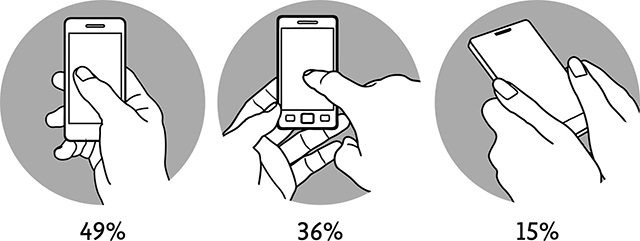
\includegraphics[width=\textwidth]{images/MobileWeb-Fitts}	
						\caption[Mobile Web - Impugnature e utilizzo] {Mobile Web - Tipi di impugnatura e percentuale di utilizzo}
						\label{fig:MobileWeb-Fitts}
					\end{figure}
					
					Come si vede dalla figura ~\ref{fig:MobileWeb-Fitts}, l'uso del pollice è preferito (75\%) e questo garantisce una \textbf{pessima precisione}. Ci sono poi delle zone di \textbf{bassa usabilità} perché raggiungibili solo allungando la mano, nel caso dei tablet peggio ancora, per questo i controlli dovrebbero essere sempre nella parte inferiore (come i controlli standard degli smartphone). Bisogna poi tenere conto che la forma dello schermo può cambiare da normale a landscape. La migliore interfaccia quindi deve tenere conto di tutti i casi e lasciare la possibilità all'utente di cambiare interfaccia.
					\subparagraph{Zone magiche}
						Riguardo le così definite \emph{zone magiche} su mobile non disponiamo di nessuna finestra. I \emph{fan menu} funzionano molto bene meno invece i \emph{pie menu} perché le dita coprono parti di schermo e quindi anche pulsanti.
					


\end{document}	